\documentclass[12pt,answers]{exam}
\usepackage{amsmath,amsfonts,amssymb,commath,mathtools,physics}
\usepackage{todonotes}
\usepackage{enumitem}
\usepackage{float}
\newcommand{\vect}[1]{\left\langle #1 \right\rangle}
\newcommand{\tcurl}{\operatorname{curl}}
\newcommand{\tdiv}{\operatorname{div}}
\newcommand{\tgrad}{\operatorname{grad}}
\newcommand{\RR}{\mathbb{R}}

\pagestyle{headandfoot}
\firstpageheadrule
\runningheadrule
\firstpageheader{Math 222}{Final Exam Version B|Solutions, Page \thepage\ of \numpages}{2018 Fall}
\runningheader{Math 222}{Final Exam Version B|Solutions, Page \thepage\ of \numpages}{2018 Fall}
\runningfooter{}{}{}

% \title{2018 Fall Calc 3 Final Version A|Solutions}
% \author{Winston Cheong}
% \date{}

\begin{document}
% \maketitle
\begin{questions}
	\question Here is a vector which you can assume has unit length:
	\begin{figure}[H]
		\centering
		\vspace{.5in}
		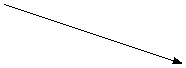
\includegraphics{graphics/2018-fall-final-vb-1.pdf}
		\vspace{.5in}
	\end{figure}
	Call this vector $\vb{u}$. Now using the same base point draw a vector $\vb{w}$ (and label it) so that the following are all satisfied:
	\begin{enumerate}[label=(\alph*)]
		\item $|\vb{w}| = 1$.
		\item $\vb{u} \cross \vb{w}$ points toward you
		\item $\vb{u} \cross \vb{w} \approx \sqrt 3/2$. (Try to make it as close as you can.)
	\end{enumerate}
	Next using the same base point again draw a vector $\vb{v}$ (and label it) so that the following are all satisfied:
	\begin{enumerate}[label=(\alph*)]
		\item $|\vb{v}| = 1$.
		\item $\vb{u} \vdot \vb{v} \approx -1/2$. (Again, do your best to get equality.)
		\item $\vb{u} \cross \vb v$ points toward you.
	\end{enumerate}
	\begin{solution}
		
		\begin{align*}
			\vb u \cross \vb w &= \| \vb u \| \|\vb w\| \sin \theta = \sqrt 3/2 \implies \theta = 60^\circ \\ 
			\vb u \vdot \vb v &= \| \vb u \| \|\vb v\| \cos \theta = -1/2 \implies \theta = 120^\circ
		\end{align*}
		so the final configuration looks like
		\begin{figure}[H]
			\centering
			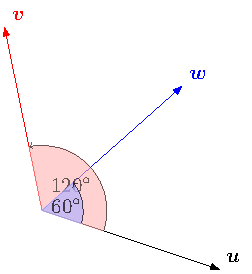
\includegraphics{graphics/2018-fall-final-vb-1-sol.pdf}
		\end{figure}
	\end{solution}

	\newpage
	\question
	Short answers\ldots Intuition and Understanding
	\begin{parts}
		\part If you are driving, then what device (or devices) in your car will be the best way to change your tangential acceleration?
		\begin{solution}
			Gas pedal \& brake
		\end{solution}

		\part What is the curvature of a circle with radius 64?
		\begin{solution}
			$\kappa = \frac{1}{64}$
		\end{solution}

		\part $f(x,y)$ is defined to equal 5 for all points on the disk $(x-1)^2 + (y-2)^2 \le 16$, to equal $-3$ for all points on the disk $(x+5)^2 + (y+8)^2 \le 4$, and to equal 0 everywhere else. Compute:
		\[
			\int_{x=-90}^{100} \int_{y=-100}^{90} f(x,y) \dif y \dif x.
		\]
		\begin{solution}
			$= 5 \cdot \pi (4^2) - 3 \pi (2^2) = \boxed{68\pi}$
		\end{solution}

		\part Will the surface integral
		\[
			\iint_{S} f(x,y,z) \dif S
		\]
		typically give you the surface area of $S$? Explain your answer in one sentence or less.
		\begin{solution}
			No. Only if $f(x,y,z) = 1$ will the integral compute the surface area of $S$.
		\end{solution}
		\part What is the average value of the function $f(x,y) = 4 + 2y$ on the rectangle $2\le x \le 6$, $1 \le y \le 3$?
		\begin{solution}
			\[
				= \frac{\int_1^3 \int_2^6 (4+2x) \dif x \dif y}{(6-2)(3-1)} 
				= \frac{\int_2^6 (4+2x) \dif x}{4}
				= \frac{\left[4x+x^2\right]_2^6}{4} = \boxed{12}
			\]
		\end{solution}
	\end{parts}

	\newpage
	\question
	Short answers\dots Definitions and Theorems
	\begin{parts}
		\part Suppose that $\nabla f(0,0) = \vect{0,0}$, and $f_{xx}(0,0)$ and $f_{yy}(0,0)$ are both negative. Do you need anything else to conclude that $(0,0)$ is a local maximum? (If yes, then what? If no, then why not?)
		\begin{solution}
			Yes, need to know that the discriminant $> 0$.
			In particular, that $f_{xx}(0,0) f_{yy}(0,0) > f_{x,y}(0,0)^2$.
		\end{solution}
		\part What does it mean (definition!) for a vector field $\vb{F}(x,y,z)$ to be incompressible?
		\begin{solution}
			$\tdiv \vb{F} = 0$.
		\end{solution}
		\part According to the theorem that we learned, if $f$ is a continuous function on a set $\Omega$, then what condition or conditions on $\Omega$ will guarantee that $f$ attains an absolute maximum and absolute minimum?
		\begin{solution}
			$\Omega$ must be closed and bounded
		\end{solution}
		\part Assume that you have been given a differentiable vector field defined on the first octant. How can you quickly tell if it is conservative?
		\begin{solution}
			Since it is defined on the entire first octant (a simply connected domain), the vector field is conservative if and only if its curl is the zero vector.
		\end{solution}
	\end{parts}

	\newpage 
	\question
	A certain differentiable function satisfies:
	\begin{enumerate}[label=(\alph*)]
		\item $f(2,-4) = 1$, and $f(-9,6)= 7$
		\item $\nabla f(2,-4) = (5,3)$, and $\nabla f = (-9,6) = (8, -\pi)$.
	\end{enumerate}
	At each of the two points in question (i.e.~at $(2,-4)$ and at $(-9,6)$) answer the following questions:
	\begin{parts}
		\part In what direction is the function increasing the fastest?
		\begin{solution}~\\
			For $(2,-4)$: $\vect{5, 3}$; \\
			For $(-9, 6)$: $\vect{8, -\pi}$.
		\end{solution}

		\part What is the rate of change in that direction?
		\begin{solution}~\\
			For $(2, -4)$: $\sqrt{25 + 9} = \sqrt{34}$; \\
			For $(-9, 6)$: $\sqrt{64+\pi^2}$.
		\end{solution}

		\part What is the directional derivative in the direction of $\vect{4,-3}$? (Note: just to be completely clear about semantics here, you are supposed to give the same directional derivative at each point. I did not ask for the directional derivative in the direction of the point $(4,-3)$.)
		\begin{solution}
			Let $\vb u = \vect{\frac45, -\frac35}$.

			For $(2,-4)$: $D_{\vb u} f(2,-4) = \nabla f(2,-4) \vdot \vb{u} = \vect{5,3} \vdot \vect{\frac45, -\frac35} = \frac{11}{5}$. \\ 
			For $(-9,6)$: $D_{\vb u} f(-9,6) = \nabla f(-9,6) \vdot \vb{u} = \vect{8, -\pi} \vdot \vect{\frac45, -\frac35} = \frac{32+3\pi}{5}$.
		\end{solution}

		\part What is the tangent plane and/or the linear approximation at each of the two points?
		\begin{solution}~\\
			For $(2,-4)$: $L(x, y) = 1 + 5(x-2) + 3(y+ 4)$\\
			For $(-9,6)$: $L(x, y) = 7 + 8(x+9) - \pi(y - 6)$
		\end{solution}
	\end{parts}

	\newpage
	\question
	Find the maximum and minimum of the function
	\[
		f(x,y) = x - 4x^2 + 3 y - 4y^2
	\]
	on the set 
	\[
		g(x,y) = x^2 + y^2 \le 40.
	\]
	Show your work carefully, and explain what you are doing. (No essays, please. Just a few short words in the right places will suffice.)
	\begin{solution}
		First, consider $g < 40$. Setting $\nabla f = 0$, and solving
		\[
			\nabla f = \vect{1-8x,3-8y} = \vb 0
		\]
		gives the critical point $(\frac18, \frac38)$.
		Next, considering $g = 40$, we solve $\nabla f = \lambda \nabla g$:
		\[
			\left\{
				\begin{aligned}
					1-8x&=2\lambda x\\
					3-8y&=2\lambda y\\
					x^2 + y^2 &= 40
				\end{aligned}
			\right.
		\]
		The first two equations give
		\[
			x = \frac{1}{8+2\lambda}\qquad y = \frac{3}{8+2\lambda}
		\]
		Substituting into the the third equation gives
		\[
			\frac{10}{(8+2\lambda)^2} = 40
			\implies \frac{1}{(8+2\lambda)^2} = 4
			\implies \frac{1}{8+2\lambda} = \pm 2
		\]
		which yields the two constrained critical points: $(2, 6)$, $(-2, -6)$.
		Evaluating $f$ on the found critical points:
		\begin{align*}
			f(\frac18, \frac38) &= \frac{5}{8} \\ 
			f(2, 6) &= -140 \\ 
			f(-2, -6) &= -180
		\end{align*}
		Thus the maximum is $\frac58$, and the minimum is $-180$.
	\end{solution}

	\newpage
	\question
	Let $S$ be the part of the set 
	\[
		z = x^2 + y^2
	\]
	which is between the planes $z=9$ and $z=16$. \\ 
	Express the surface area for $S$ as an iterated integral (i.e.~a double or triple integral) over a subset of $\RR^2$ or $\RR^3$ which has \textbf{constant} bounds of integration. (i.e.~it should be over a rectangular solid or a rectangle in the domain in which you are finally integrating.) You do \textbf{NOT} need to find this integral.
	\begin{solution}
		The set $S$ can be parametrized by 
		\[
			G(r, \theta) = (r\cos \theta, r\sin\theta, r^2) 
			\qquad 3 \le r \le 4, 
			\ 0 \le \theta \le 2\pi
		\]
		We can then compute
		\begin{align*}
			\vb{N} = G_r \cross G_\theta 
			&= \vect{\cos \theta, \sin\theta, 2r} \cross \vect{-r\sin\theta, r\cos\theta, 0}  \\ 
			&= \vect{-2r^2\cos\theta, -2r^2\sin\theta, r}
		\end{align*}
		and
		\[
			\|\vb{N}\| = \sqrt{4r^4+r^2}
		\]
		The surface area of $S$ can thus be computed as the surface integral
		\[
			\iint_S 1 \dif S  = \boxed{\int_0^{2\pi} \int_3^4 \sqrt{4r^4+r^2} \dif r \dif \theta}
		\]
	\end{solution}

\newpage
\question
Let $C$ be the curve given by
\[
	\vb{r}(t) = \left(t \cdot \cos(5\pi t),
	\frac{t^3}{4+t^2},
	t + \sin(5\pi t)
	\right),
\]
with $0 \le t \le 2$. Compute the following integral:
\[
	\int_C \vect{y, x, 3z^2} \vdot \dif \vb{r}.
\]
\begin{solution}
	Note that the vector field $\vb{F} = \vect{y, x,3z^2}$ is conservative, with potential function $f = xy + z^3$.
	Hence by the Fundamental Theorem for Line Integrals, 
	\begin{align*}
		\int_C \vb{F} \vdot \dif \vb{r}
		 & = f(\vb{r}(2)) - f(\vb{r}(0)) \\
		 & = f(2,1,2) - f(0,0,0)   \\
		 & = 2+8-0
		= \boxed{10}
	\end{align*}
\end{solution}

	\newpage
	\question
	Let $Q$ be the set of points within the set:
	\[
		\{ (x,y,z) : x^2+y^2+z^2 \le 9, \quad \text{and } 0 \le y \}
	\]
	and let $\partial Q$ be the boundary of this set. If $\vb{n}$ is the outward unit normal to this region, then compute:
	\[
		\iint_{\partial Q} (\cos(z^4), y^2, \sin(x^4)) \vdot \vb{n} \dif S.
	\]
	\begin{solution}
		By the divergence theorem, 
		\[
			\iint_{\partial Q} \vb{F} \vdot \dif \vb{S} = \iiint_{Q} \tdiv \vb F \dif V
		\]
		so 
		\begin{align*}
			\iint_{\partial Q} (\cos(z^4), y^2, \sin(x^4)) \vdot \vb{n} \dif S
			&= \iiint_Q 2y \dif V
		\end{align*}
		Evaluating this integral in spherical coordinates,
		\begin{align*}
			\iiint_{Q} 2y \dif V 
			&= \int_{0}^{\pi} \int_0^\pi \int_0^3 2 \rho \sin\varphi \sin\theta \cdot \rho^2 \sin\varphi \dif \rho \dif \varphi \dif \theta\\
			&= \int_0^3 2\rho^3 \dif \rho 
			\cdot
			\int_{0}^{\pi} \sin\theta \dif \theta
			\cdot
			\int_0^\pi \sin^2\varphi \dif \varphi 
			\\
			&= \left[ \frac{\rho^4}{2} \right]_0^3
			\cdot
			\left[-\cos\theta\right]_0^\pi
			\cdot
			\left[\frac12 \varphi - \frac14 \sin2\varphi\right]_0^\pi
			\\
			&= \frac{81}{2} \cdot (1+1) \cdot (\frac\pi2 - 0 - 0) 
			\\
			&= \boxed{\frac{81\pi}{2}}
		\end{align*}
	\end{solution}

	\newpage
	\question
	Let $E$ be the subset of
	\[
		z = x^2 + y^2
	\]
	which also satisfies 
	\[
		z \le 16, \qquad x \ge 0, \qand y \le 0.
	\]
	Express
	\[
		\iint_E y^2 \dif S
	\]
	as an iterated integral (i.e.~a double or triple integral) over a subset of $\RR^2$ or $\RR^3$. You do \textbf{NOT} need to find this integral.
	\begin{solution}
		The set $E$ can be parametrized by 
		\[
			G(r, \theta) = (r \cos \theta, r\sin\theta, r^2) 
			\qquad 0 \le r \le 4, 
			\quad -\frac\pi2\le \theta \le 0
		\]
		Then we can compute
		\begin{align*}
			\vb{N} = G_r \cross G_\theta 
			&= \vect{\cos \theta, \sin\theta, 2r} \cross \vect{-r\sin\theta, r\cos\theta, 0}  \\ 
			&= \vect{-2r^2\cos\theta, -2r^2\sin\theta, r}
		\end{align*}
		and
		\[
			\|\vb{N}\| = \sqrt{4r^4+r^2}
		\]
		Which allows to rewrite the integral as
		\[
			\iint_E y^2 \dif S 
			= \boxed{\int_{-\frac\pi2}^0 \int_0^4 r^2 \sin^2\theta \cdot \sqrt{4r^4+r^2} \dif r \dif \theta}
		\]
		
	\end{solution}

	\newpage
	\question
	Let $E$ be the part of the set
	\[
		\sqrt{x^2+y^2} \le z \le 3
	\]
	that also satisfies
	\[
		x \le 0.
	\]
	Find 
	\[
		\iiint_{E} x \dif V.
	\]
	\begin{solution}
		The inequaltiy can be reexpressed as 
		$0 \le r \le z \le 3$. 
		The bounds for the variables are
		\[
			\theta \in [\frac\pi2, \frac{3\pi}{2}] 
			\qquad 
			r \in [0,3]
			\qquad
			z \in [r,3]
		\]
		$E$ is half of a solid cone.
		The integral can be written in cylindrical coordinates as
		\begin{align*}
			\int_{\frac\pi2}^{\frac{3\pi}{2}} \int_0^3 \int_r^3 r \cos \theta \cdot r \dif z \dif r \dif \theta
			&= \int_{\frac\pi2}^{\frac{3\pi}{2}} \cos\theta \dif \theta \cdot \int_0^3 \int_r^3 r^2 \dif z \dif r \\
			&= \left[ \sin\theta\right]_{\frac\pi2}^{\frac{3\pi}{2}} 
			\cdot \int_0^3 r^2 (3-r) \dif r \\
			&= (-1-1) \cdot \left[r^3 - \frac{r^4}{4}\right]_0^3 \\
			&= -2\left(27 - \frac{81}{4}\right)
			= \boxed{-\frac{27}{2}}
		\end{align*}
	\end{solution}

\end{questions}

\end{document}
